\subsection{Mixed Reality und HoloLens}
\label{sec-2-1}

\subsubsection{Mixed Reality}
\label{sec-2-1-1}
\fbox{
	\parbox{\linewidth}{
		\textit{Ziel des Kapitels:}\\
		Begriffsklärung und Einordnung von AR,MR,VR in das Virtual Continuum. Wichtig für die Einordnung von MR in Education in Kap. \ref{sec-2-2}.\\
}}

\begin{figure}[h!]
	\centering
	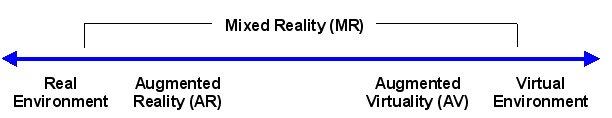
\includegraphics[width=0.9\textwidth]{images/virtual_continuum.png}
	\caption{Virtual Continuum eingeführt von Paul Milgram \cite{Milgram94}}
	\label{img:virtual_continuum}
\end{figure}

\begin{itemize}
	\item Kontinuierliches Spektrum zwischen real und virtuell
	\item MR ist Bereich zwischen völlig real und völlig virtuell, d.h. schließt AR und AV ein
	\item (optional) Einordnung von Beispielen HUD, Snapchat, Fragments, Oculus Rift
	\item Leistungssteigerung im Hardwarebereich und Fortschritte bei AI führt zur Verfügbarkeit von Devices von AR bis VR, daher sehr aktuelles Thema, viel Potential
\end{itemize}


\subsubsection{HoloLens}
\label{sec-2-1-2}
\fbox{
\parbox{\linewidth}{
	\textit{Ziel des Kapitels:}\\
	HoloLens und Mixed Reality Toolkit mit ihrer Technik und Interaktionsweise vorstellen.
}}\\

\textbf{Hardware}\\
\begin{itemize}
	\item HMD mit stereoskopischem see through display, je ein Display pro Auge in festem Abstand, 32 Grad FOV
	\item 60hz upscale zu 240hz, jede Farbe einzeln sequenziell, pro Anwendungsframe also 3 Farbframes mit Laserlicht
	\item Inside out tracking mit IMU, 2x IR und 2x Stereo Kamera, 1x 2MP / HD Kamera, 4 Mikrofone, Ambient Light sensor
	\item Weitere Hardware und Software Specs
\end{itemize}	

\textbf{Software und Interaktion}\\
\begin{itemize}
	\item Windows 10 Holographic und UWP Apps
	\item Gesten- und Spracherkennung von einigen Handgesten bzw. englischen Wörtern inbegriffen
	\item Raumerkennung und räumliches Verständnis vorhanden
	\item Mixed Reality Toolkit mit wichtigen Funktionen und Beispielen
	\item Entwicklung mit Unity unterstützt
\end{itemize}


\textbf{Implikationen für Anwendungsdesign (kurz)}\\
Genannte technische Details haben Auswirkung auf Nutzung und Design von Anwendungen
\begin{itemize}
	\item Stark spiegelnde oder transparente Materialien ungünstig für das Tracking
	\item Kein Schwarz darstellbar, Helligkeit im Raum relevant, Brille nur in Räumen zu verwenden
	\item Strenge Limitierung von Resourcen für Anwendung, da 60 FPS gehalten werden sollten, also keine komplexen Berechnungen möglich
	\item Abstand, Geschwindigkeit und Größe der Objekte wichtig, Blickwinkel
\end{itemize}
